\chapter{A Design Space for Diminished Reality under Compositing Constraints}

\section{The Compositing Constraint}

Chapter 2 established that diminished reality (DR), the selective removal or attenuation of
real-world visual information \citep{mori2017}, has a substantial conceptual literature and a thin
implementation record on consumer hardware. This chapter asks the technical half of the
dissertation's question: what degree of diminishment control is actually achievable on a consumer
video-see-through (VST) headset, without operating-system-level access to the passthrough layer?

The answer is not a single number but a structured design space, and this taxonomy is Contribution
C1. The central claim is that on a platform such as the Meta Quest 3, the feasibility of any DR
effect is decided almost entirely by \textbf{which layer of the compositing stack an application is
permitted to touch}, and that these permissions stratify into three tiers with sharply different
capabilities and costs.

On Quest 3 the reconstructed view of the real world that the user experiences, the system
passthrough, is produced and owned by the operating system. An application \textbf{cannot read,
modify, or subtract from the passthrough layer. It can only composite content on top of it.} The
passthrough image is never exposed to application shaders as a texture. It is composited
\textit{behind} application content by the OS compositor, at a stage of the pipeline applications do
not reach. The naive formulation of subtractive DR, sample the passthrough pixel, darken it, write it
back, is therefore not merely difficult on this platform. It is architecturally impossible.

This is a deliberate privacy and safety boundary rather than an incidental limitation, and it is
shared in stronger form by the other major consumer platform. On Apple Vision Pro camera pixels are
unavailable to consumer applications entirely, since raw camera access requires an enterprise-only
entitlement incompatible with App Store distribution, and the only world-appearance control offered
is a global, non-spatial surroundings dimming effect \citep{apple2024}. On true optical see-through
(OST) glasses the constraint is harsher and physical rather than administrative. An additive display
can only \textit{add} light to the optical path. It can superimpose brightness but cannot remove
photons arriving from the world, so darkening is unavailable without auxiliary hardware such as
per-pixel dimming layers \citep{itoh2021}.

The motivation for the boundary predicts its persistence. The passthrough image is a continuous
camera view of the user's home, workplace, and bystanders. Granting arbitrary applications read
access to it is a privacy exposure, and granting write access is a safety exposure, because an
application could imperceptibly alter the user's view of the physical world they are walking through.
Both concerns strengthen rather than weaken over time, so research that assumes future
read-modify-write access to system passthrough is betting against the platform vendors' incentives.
This dissertation makes the opposite bet. It treats the constraint as permanent and asks what can be
built inside it, which is what gives the resulting design space its claim to durability.

Subtractive attention guidance must therefore be \textit{synthesised} on consumer VST hardware
through whatever compositing rights the platform does grant. Figure~\ref{fig:stack} shows the three
layers of the stack and which of them each tier of access is permitted to touch.

\begin{figure}[htbp]
\centering
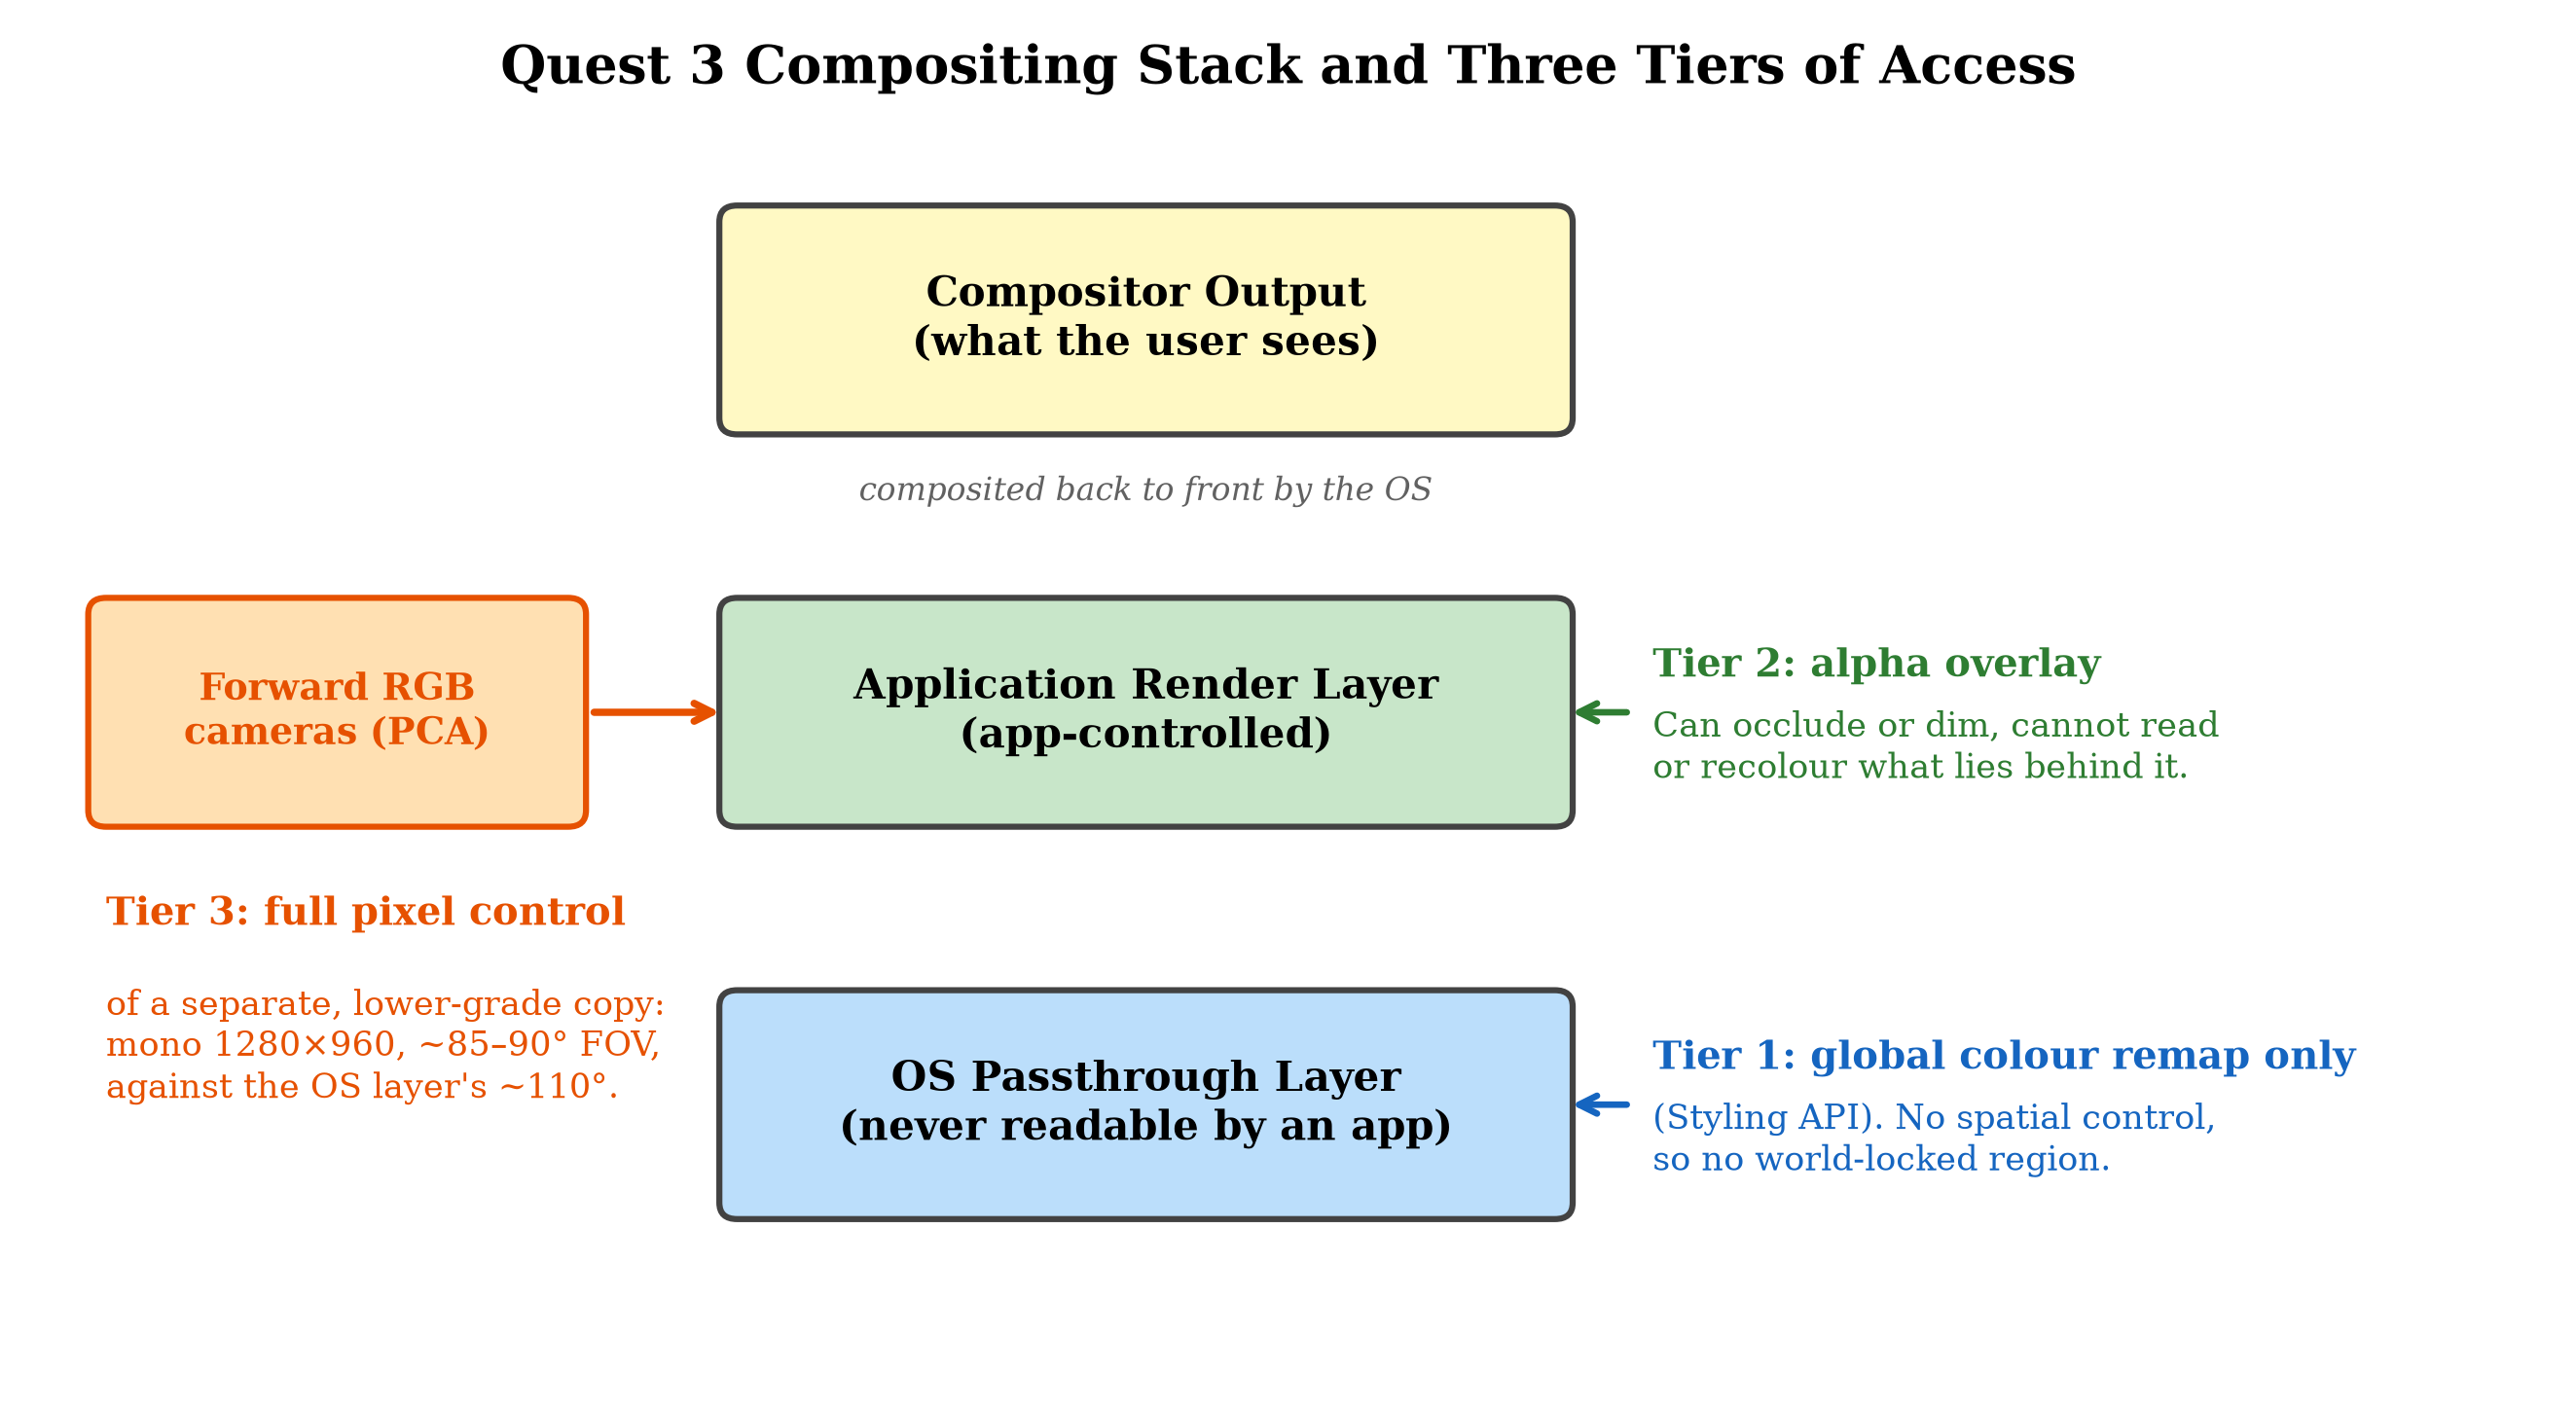
\includegraphics[width=\linewidth]{content/figures/fig_compositing_stack.png}
\caption{The Quest 3 compositing stack and the three tiers of access.}
\label{fig:stack}
\end{figure}

\section{The Three-Tier Access Taxonomy}

The Quest 3 grants applications three distinct kinds of access relevant to DR, summarised in
Table~\ref{tab:tiers}.

%% Five p-columns leave only \textwidth minus 5*2*\tabcolsep for content, so \tabcolsep is
%% halved and the widths sum to 0.90 rather than 0.94. Without both the row is 33pt over.
\begingroup
\setlength{\tabcolsep}{4pt}\small
\begin{longtable}{p{0.13\textwidth}p{0.20\textwidth}p{0.17\textwidth}p{0.26\textwidth}p{0.14\textwidth}}
\caption{Diminished-reality capability by compositing-access tier on Quest 3.}
\label{tab:tiers} \\
\hline
\textbf{Tier} & \textbf{Access mechanism} & \textbf{Achievable DR} & \textbf{Ceiling / cost} & \textbf{Modes located here} \\
\hline
\endfirsthead
\hline
\textbf{Tier} & \textbf{Access mechanism} & \textbf{Achievable DR} & \textbf{Ceiling / cost} & \textbf{Modes located here} \\
\hline
\endhead
\textbf{1: OS pass\-through styling} &
\texttt{OVRPass\-through\-Layer} Styling API: brightness / contrast / saturation scalars, 3D colour look-up tables, edge tint &
\textbf{Global colour remapping only.} Whole-layer desaturation, tinting, posterisation &
No blur. No per-pixel or spatial masks. No world-locked regions. Layer can never be read. Surface-projected passthrough deprecated at SDK v83 &
Not applicable (bounding case) \\
\hline
\textbf{2: Overlay compositing} &
Application draws alpha-blended geometry in front of the passthrough layer &
Dimming, blackout, occlusion. A shaped \textit{absence} of overlay passes OS-native passthrough through untouched &
Can only attenuate or occlude reality. Cannot recolour, blur, or filter it &
Soft Dark, Hard Dark, GranulatedPeriphery, SpotLift. The focus window itself \\
\hline
\textbf{3: Camera re-render (PCA)} &
Passthrough Camera Access: the raw forward camera feed as a GPU texture, with intrinsics and pose &
Arbitrary per-pixel manipulation: blur, desaturation, salience re-grading, glare compression &
Mono 1280$\times$960 at $\sim$85–90$^{\circ}$ horizontal FOV vs the $\sim$110$^{\circ}$ OS view. Added latency. Binocular-fusion burden (Chapter 4). Sustained on-device processing is thermally bounded &
SignPop (evaluated, built on the ColorPop pipeline), ColorPop, Blur (superseded), Chromatic\-Cool, Conspicuity\-Squeeze, Outlined\-Dark \\
\hline
\end{longtable}
\endgroup

\subsection{Tier 1: the styling ceiling}

Tier 1 deserves precision because it prevents an overclaim this dissertation must not make. It is
\textit{not} true that nothing can be done to the system passthrough layer. Meta's Passthrough
Styling API allows an application to apply brightness, contrast and saturation adjustments, full 3D
colour look-up tables, and edge tinting to the layer as a whole \citep{meta2024a}. A global
desaturation of the entire visual field, one conceivable DR primitive, is achievable at Tier 1
without touching a camera pixel.

What Tier 1 categorically lacks is \textbf{spatial control}. Every styling operation applies to the
whole layer uniformly. There is no mechanism for per-pixel masks, gradients, world-locked regions, or
any effect that treats one part of the visual field differently from another. The one historical
exception, surface-projected passthrough, allowed passthrough to be projected onto
application-defined geometry with per-surface styling. It was deprecated at SDK v83 and is
unavailable going forward. Attention guidance is \textit{definitionally} spatial, since its entire
purpose is to treat the focus region differently from the periphery, so Tier 1 alone cannot implement
any mode in this dissertation. \textbf{The absence of spatial control, not the absence of control, is
the finding.}

\subsection{Tier 2: diminishment by occlusion}

Tier 2 is ordinary alpha compositing. The application draws translucent or opaque geometry in front
of the passthrough layer. Because the VST display is an opaque screen whose every pixel the
compositor ultimately controls, an overlay can darken the apparent world without limit, up to and
including full blackout, which is physically impossible on additive OST optics. The constraint runs
the other way: a Tier-2 overlay knows nothing about the pixels behind it, so it can attenuate or
occlude reality but cannot recolour, sharpen, blur, or respond to its content.

Two modes live entirely at Tier 2. \textbf{Soft Dark} composites a uniform black overlay at up to
75\% opacity across the periphery. \textbf{Hard Dark} takes the same overlay to full opacity. Both
leave a shaped hole, the world-locked focus window, through which untouched OS passthrough remains
visible.

That hole is the load-bearing architectural insight of the whole system, and it is worth stating in
its general form. \textbf{At Tier 2, the highest-fidelity rendering of reality is an absence of
rendering.} Inside the focus window nothing is drawn at all, so the user receives OS passthrough at
its full native quality, full $\sim$110$^{\circ}$ field of view, and zero added latency, precisely
where they are being asked to direct their attention. The manipulation is confined to the periphery,
where visual acuity is lowest and quality loss matters least. This inverts the naive design of
re-rendering the whole view from the camera feed and accepting camera-grade quality everywhere, and
it is why the system escapes the passthrough-acuity ceiling exactly where task performance depends on
seeing well. Alpha punch-through as a mechanism is documented platform practice \citep{meta2024b} and
shipped commercially in Immersed's Passthrough Portals \citep{immersed2022}, but in all found prior
uses the hole reveals passthrough \textit{surrounded by virtual content}. Using the hole as the focus
region of a diminished periphery is, per Section~\ref{sec:novelty}, unprecedented.

\subsection{Tier 3: full pixel control at a price}

Tier 3 is the Passthrough Camera Access (PCA) API \citep{meta2025}, which since early 2025 exposes
the headset's forward RGB camera feed to applications as a GPU texture together with camera
intrinsics and pose. At Tier 3 the application is no longer manipulating a proxy for reality. It
holds camera pixels and can apply arbitrary per-pixel computation: Gaussian blur, luminance-weighted
desaturation, hue-selective salience re-grading, glare compression.

The price is paid in four currencies. \textbf{Resolution and field of view}: the accessible feed is a
single mono stream at 1280$\times$960 covering roughly 85–90$^{\circ}$ horizontally, against the OS
passthrough's $\sim$110$^{\circ}$ stereo view, so a Tier-3 re-render is categorically lower-fidelity
than what the user would otherwise see. \textbf{Latency}: the application-side pipeline of camera
capture, texture upload, shader, and display adds delay the OS passthrough path, with its dedicated
reprojection, does not exhibit. \textbf{Binocular fusion}: the feed is monocular, and presenting it
convincingly to two eyes is non-trivial, since the naive approach measurably fails (Chapter 4).
\textbf{Thermal budget}: sustained on-device processing of the camera stream is bounded. The only
published work to quantify this class of hardware for PCA-style live compositing is a
simulation-based feasibility study projecting 720p30 operation with thermal throttling after five to
ten minutes \citep{laghari2025}. That figure is projected rather than measured, since no benchmark
ran on physical hardware, but it means Tier-3 modes are on today's hardware modes for sessions rather
than workdays.

\subsection{The hybrid: composing Tier 2 and Tier 3}

The tiers are not mutually exclusive, and the most capable configuration this work demonstrates is a
composite. The PCA camera feed, shader-processed, is rendered onto a head-centred sphere as the
periphery at Tier 3, with the world-locked focus window left transparent so native OS passthrough
shows through the hole by Tier 2's absence trick. The user experiences full-fidelity reality inside
the window, seamlessly surrounded by a re-graded interpretation of reality outside it. This exploits
the quality and field-of-view asymmetry between the two layers rather than suffering it.
Figure~\ref{fig:hybrid} separates the composite into its layers and shows the single view they fuse
into. The implementation is Chapter 4's subject.

\begin{figure}[htbp]
\centering
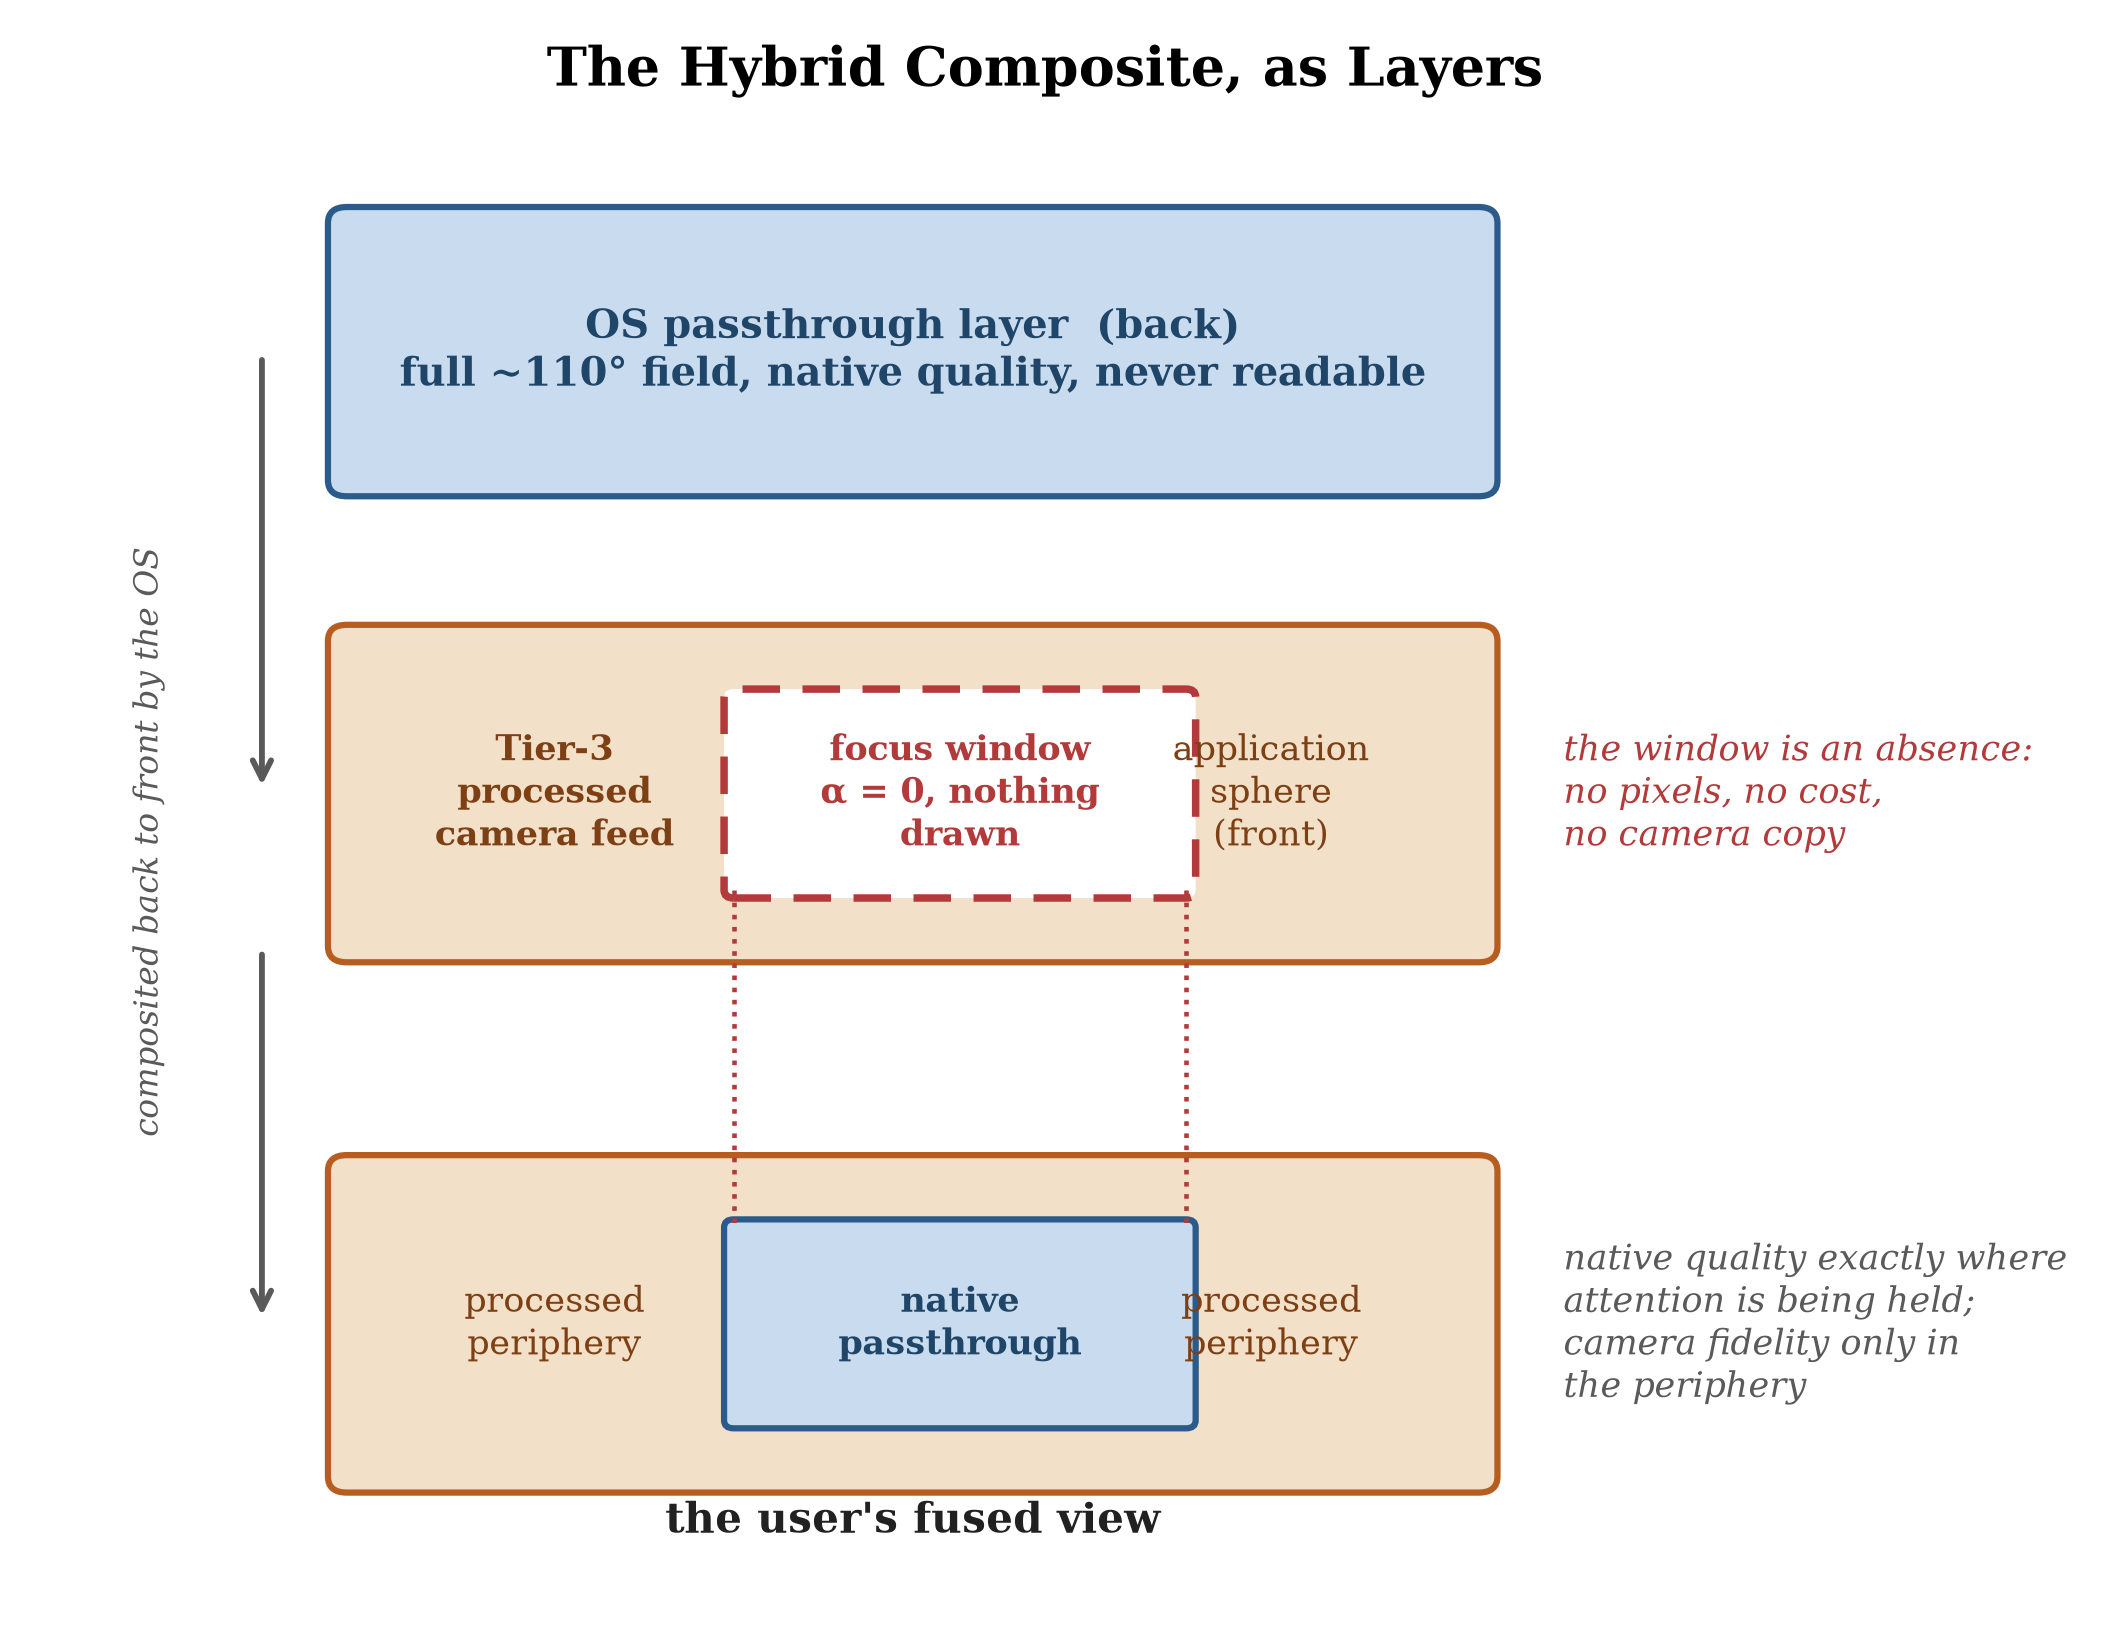
\includegraphics[width=\linewidth]{content/figures/fig_hybrid_exploded.png}
\caption{The hybrid composite, shown as exploded layers.}
\label{fig:hybrid}
\end{figure}

\section{What Is Impossible, and Why It Matters}

A design space is defined as much by its walls as by its rooms. Three impossibilities structure
everything above.

\begin{itemize}
\item \textbf{No read access, at any tier, to the pixels the user actually sees.} Even Tier 3
supplies a different, lower-grade copy of reality rather than the passthrough image itself. Any
effect that must respond to what the user sees, such as content-adaptive dimming or saliency-weighted
attenuation \citep{lu2012}, can respond only to the camera proxy.
\item \textbf{No spatial modulation of the native layer.} The full-quality view can be revealed or
hidden at Tier 2 but never partially processed. A mode that blurs the real passthrough periphery,
arguably the perceptually gentlest DR primitive per the foveated-rendering literature
\citep{patney2016}, cannot exist on this platform except via the Tier-3 copy.
\item \textbf{No subtraction on OST.} The entire Tier-2 family is VST-specific, for the physical
reason given in Section 3.1. What does and does not transfer is taken up in the conclusion.
\end{itemize}

These walls explain the system's shape. The dark modes exist because attenuation-by-overlay is the
only manipulation available at native quality. ColorPop exists because re-grading requires pixels,
and pixels are only available as the Tier-3 copy. The window-as-absence exists because it is the sole
mechanism delivering native fidelity \textit{and} spatial selectivity simultaneously. Had the
platform offered read-modify-write access to the passthrough layer, none of this architecture would
be necessary. That counterfactual is what makes the taxonomy transferable: any future platform can be
located in it by asking which of the three walls it removes.

\section{Design Axes and the Placement of the Modes}

Three trade-off axes fall out of the taxonomy, and the modes carried into the study were chosen to
span them.

\textbf{Fidelity versus control.} Tier 2 offers native fidelity with a single degree of freedom,
attenuation. Tier 3 offers unlimited control at camera-copy fidelity. Hard Dark and Soft Dark sit at
the fidelity pole, since the periphery they show, when they show it, is real passthrough merely
darkened. SignPop sits at the control pole, since its periphery is a synthetic re-grading of the
camera copy.

\textbf{Suppression versus awareness.} Hard Dark removes the peripheral signal entirely: maximal
distractor suppression, zero residual awareness. Soft Dark attenuates to $\sim$75\% opacity, so
peripheral events remain detectable through the veil. SignPop suppresses selectively, dimming the
red, orange and green signal band less than other colours by default and lifting that band to full
visibility once a signal lamp or sign is confirmed (Chapter 4, Section 4.5). The study's safety
hypothesis lives on exactly this axis. The axis matters because the literature puts a real cost at
its far end: users asked what they want from diminishment prefer partial attenuation over complete
removal \citep{cheng2022}, and studies of DR in working contexts find the focus gain paired with a
situational-awareness risk \citep{murph2021,mclaughlin2025}. That is why the family keeps a graded
point between untouched vision and full blackout, and why the evaluation measures peripheral
awareness rather than assuming it survives.

\textbf{Deployability versus capability.} Soft Dark and Hard Dark run without the camera pipeline at
all, since their shader path samples no texture. They draw negligible GPU power, measured on device
at parity with an empty passthrough scene (Chapter 4, Section 4.11), require no camera permission,
and face no thermal ceiling, so they are deployable for hour-long sessions today. SignPop inherits
Tier 3's full cost structure.

Together, off $\rightarrow$ Soft Dark $\rightarrow$ Hard Dark forms a single-variable intensity ladder
(overlay alpha 0 $\rightarrow$ 0.75 $\rightarrow$ 1.0), while SignPop extends the space along the
orthogonal control axis. Figure~\ref{fig:axes} places the three on both axes, with deployability
shown alongside.

\textbf{One of the three was never placed in front of a participant.} Soft Dark occupies the midpoint
of the attenuation ladder, and its 75\% ceiling is Cheng et al.'s partial-attenuation preference
implemented as a number, but the session budget did not allow a third exposure and it was cut
(Chapter 5). This dissertation therefore reports no participant data on Soft Dark of any kind. Its
place here rests on design-space grounds and on its shader path, never on evidence about how it is
experienced. Every subsequent claim about it is a claim about the design space, not about people.

\begin{figure}[htbp]
\centering
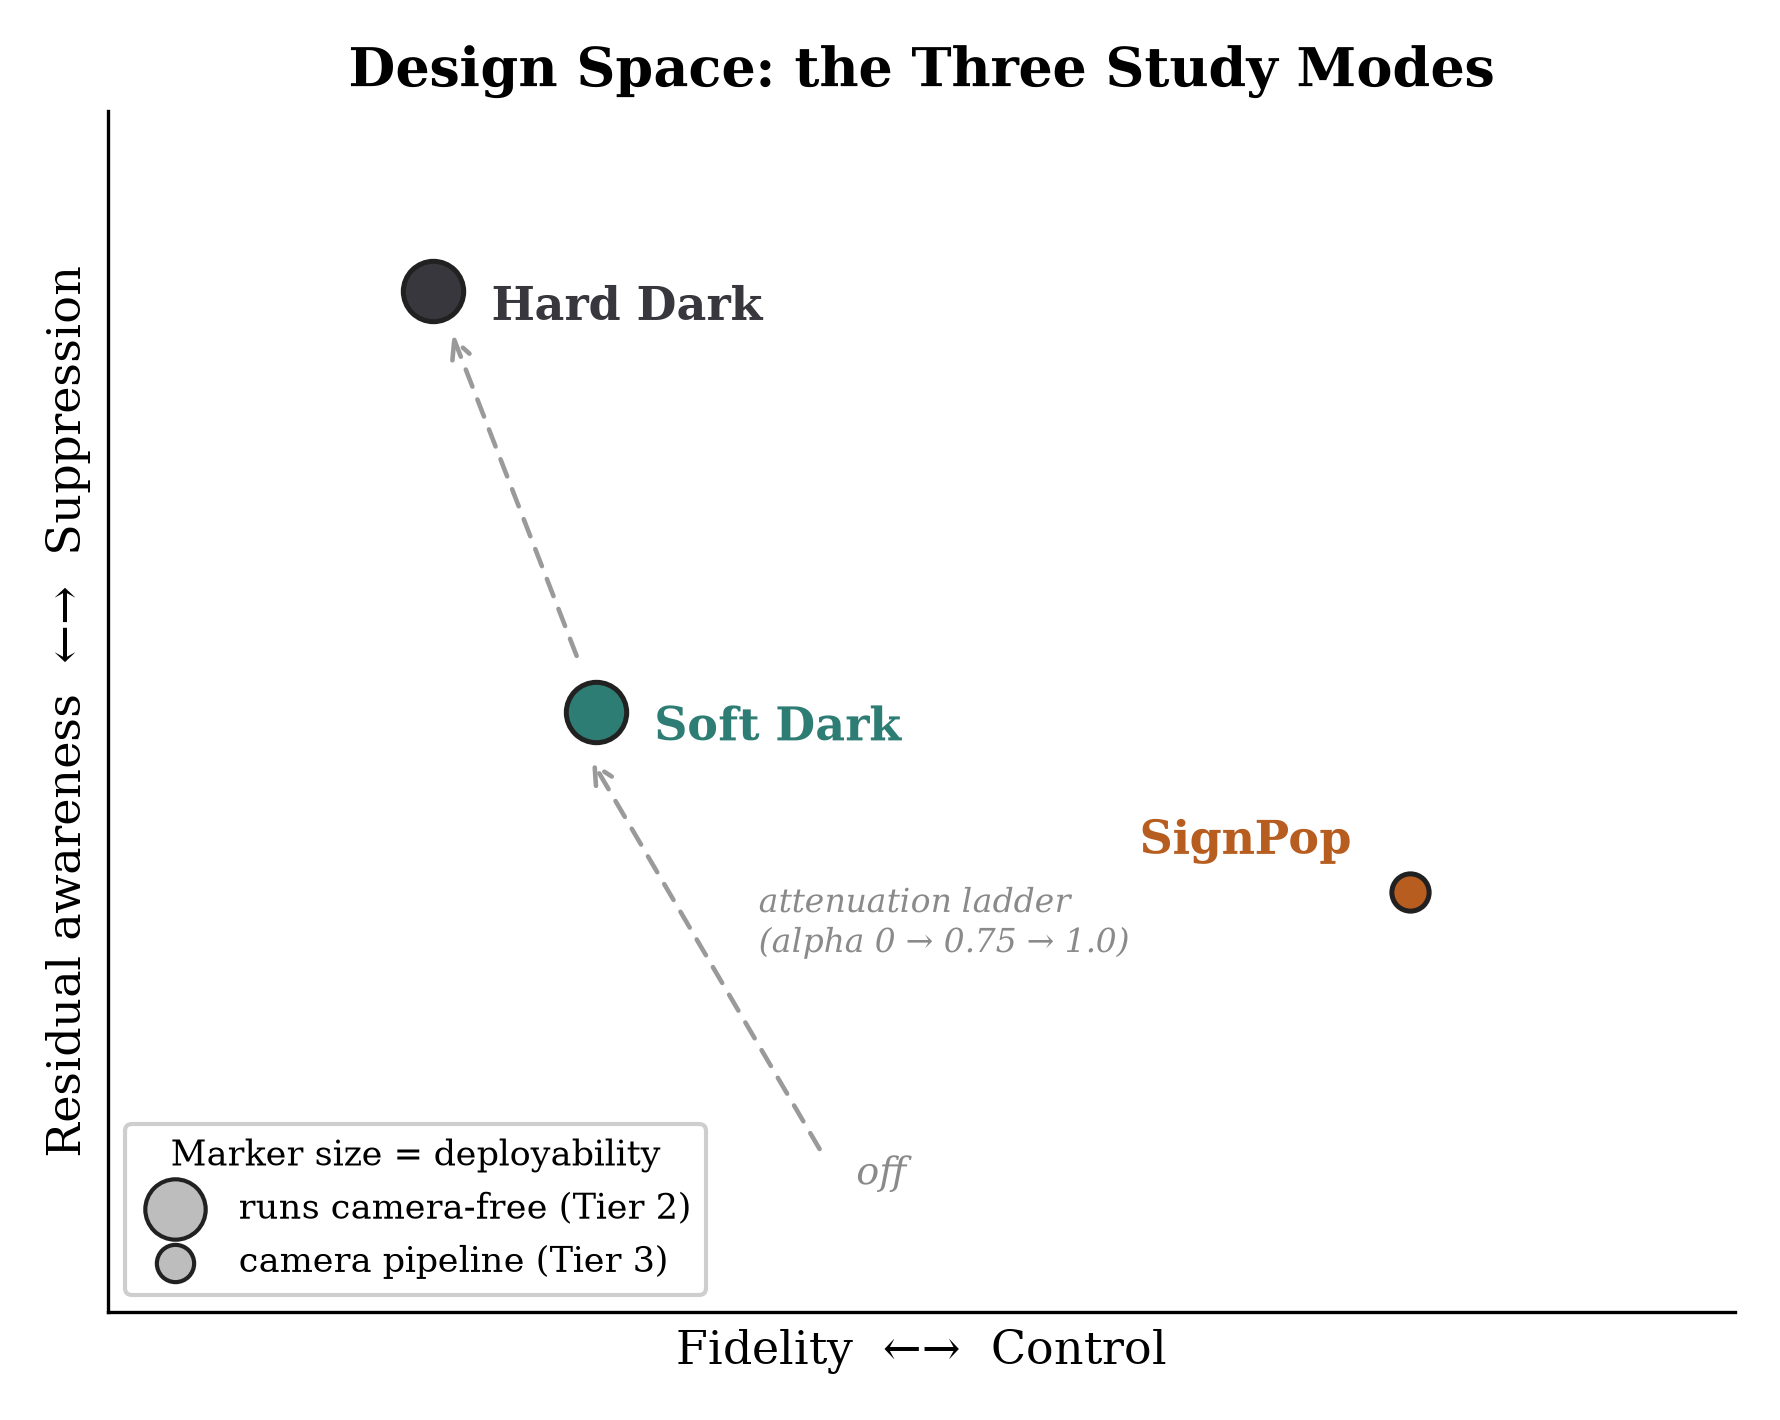
\includegraphics[width=0.75\linewidth]{content/figures/fig_design_axes.png}
\caption{Two-axis plot (fidelity/control $\times$ suppression/awareness) with the three modes placed, deployability annotated.}
\label{fig:axes}
\end{figure}

These three are not the whole family. Ten peripheral treatments were built, and the remaining seven
fill in the same two axes at points the study had no budget to test (Chapter 4, Section 4.5.3). They
also divide cleanly along the tier boundary, which is the best evidence the boundary is real rather
than imposed. Four modes never read a camera pixel and are therefore Tier 2, including SpotLift,
whose focus-window brightness lift exists only in the video path because OS passthrough cannot be
brightened. The other six read the camera feed and are therefore Tier 3. The tiers were not fitted to
three convenient examples. They were derived from building the whole family and finding that every
member's ceiling was set by the tier it had to run at.

A fourth dimension deserves naming even though this dissertation treats it as design rather than as
an experimental factor: \textbf{time}. Every mode has temporal behaviour, a formation transition when
the window locks, a fade-out when the head moves fast, a fade-in when it settles. The literature
review found these transition mechanics essentially unstudied in DR, since prior work evaluates
diminishment as a static state rather than as something that arrives, yields, and returns. The system
therefore exposes every temporal parameter as tunable, and a controlled study of DR transition
dynamics is identified in the conclusion as future work seeded by this design space rather than
resolved by it.

\section{Novelty Position}
\label{sec:novelty}

The claims of this chapter are calibrated against the structured prior-art search reported in
Chapter 2, Section 2.5.2. Three verdicts matter here.

\begin{enumerate}
\item \textbf{The hybrid composite}, system passthrough revealed through a window in a live
shader-processed camera-feed sphere: \textit{nothing found}. No paper, product, or open-source
project, for any purpose.
\item \textbf{Peripheral passthrough manipulation for attention guidance on a standalone consumer
HMD}: \textit{nothing found as an implemented system}. The nearest work is concept-level or
differently situated. \citet{mclaughlin2025} evaluate DR distraction-attenuation entirely inside VR
simulation. The DIS 2026 ADHD co-design study is formative, with no prototype. DiminishAR and the
CHI 2026 Vision Pro study target specific objects or persons with occlusion rather than the
periphery. \citet{sutton2022} modulate real-world saliency but on a bench-mounted optical see-through
rig that can only add light.
\item \textbf{A dark peripheral vignette over passthrough}: \textit{near precedent, no direct
precedent}. Quest OS v67's Theatre View ships an adjustable peripheral dimming vignette, but
explicitly not over passthrough. Vision Pro's surroundings dimming is global rather than windowed.
\end{enumerate}

Each constituent mechanic, taken alone, has documented precedent that this dissertation cites rather
than claims: camera-feed geometry with GPU effects \citep{coviello2025}, a head-centred fade sphere
revealing passthrough \citep{meta2024c}, alpha punch-through windows \citep{meta2024b,immersed2022},
OS peripheral dimming in immersive mode \citep{meta2024d}, and saliency modulation of reality on OST
hardware \citep{sutton2022}. The defensible novelty claim is therefore precisely bounded: \textbf{the
composite}, native passthrough through a world-locked focus window in an effect-processed camera-feed
periphery, exploiting the quality and field-of-view asymmetry between layers, \textbf{applied to
peripheral attention guidance on a consumer standalone headset}, together with the world-direction
fusion sampling that makes the mono feed binocularly viewable. An alpha-blended dark overlay, by
itself, is just compositing, and is not claimed as novel. Should a refresh search before submission
surface a concurrent system, the claim degrades gracefully to independent invention with a
characterised design space, which is why it is worded around the space rather than the trick.

Two adjacent patents \citep{patents} describe claim-level ideas in this territory: attenuating
external stimuli while preserving spatial awareness, and blurred external video feeds composited into
VR. Neither shows evidence of implementation. They are noted for completeness.

\section{Summary}

On consumer VST hardware, diminished reality is not one problem but three, stratified by compositing
access: a colour-only, spatially blind styling tier, an attenuation-and-occlusion overlay tier whose
most powerful move is a shaped absence, and a full-control camera-copy tier that pays in fidelity,
latency, fusion and heat. The study modes span the space this stratification creates, the hybrid
composite exploits the asymmetry between its tiers, and the walls of the space, no reads, no spatial
modulation of the native layer, no subtraction on OST, are findings in their own right. Chapter 4
descends from this map into the machine.
